\documentclass[fleqn]{article}
\usepackage{amsmath}
\usepackage{amsfonts}
\usepackage{float}
\usepackage{pgfplots}
\usepackage{pgfplotstable}
\pgfplotsset{compat=1.17}

\title{Soluciones Estadística Descriptiva}
\author{Juan Rodriguez}

\begin{document}
	\maketitle
	\section{Solución Problema 1}
	\begin{itemize}
		\item Media Yodo: $\bar{x} = \frac{\sum_{i=1}^n x_i}{n} = \frac{1307.5}{14} = 93.39$ gr de Yodo
		\item Media Cetano: $\bar{y} = \frac{\sum_{i=1}^n y_i}{n} = \frac{779.2}{14} = 55.66$ 
		\item Varianza Yodo: $s_x^{2} = \frac{\sum_{i=1}^n x_i^{2}}{n} - \bar{x}^{2} = \frac{128913.93}{14} - 93.39^{2} = 486.45$ $s_x = 22.06$
		\item Varianza Cetano: $s_y^{2} = \frac{\sum_{i=1}^n y_i^{2}}{n} - \bar{y}^{2} = \frac{43745.22}{14} - 55.66^{2} = 26.62$ $s_y = 5.16$
		\item Covarianza: $s_{xy} = \frac{\sum_{i=1}^n x_i y_i}{n} - \bar{x} \bar{y} = \frac{71347.3}{14} - (93.39 \cdot 55.66) = -101.85$
	\end{itemize}
	a) Nos piden predecir el numero de cetano (Y) sabiendo que tiene un índice de yodo de 115 (X). Por lo tanto, usamos una recta $Y | X$ \\
	\[
	y - \bar{y} = \frac{s_{xy}}{s_x^{2}} (x - \bar{x}) \rightarrow y - 55.66 = -\frac{101.85}{486.45} (x - 93.39) \rightarrow y = -0.21x + 75.27
	\]
	\[
	y = -0.21(115) + 75.27 = \boxed{51.12}
	\]
	El numero de cetano teniendo un indice de yodo de 115 es 51.12 \\
	b) Una medida de bondad del ajuste nos la da el coeficiente de correlación de Pearson
	\[
	r = \frac{s_{xy}}{s_x \cdot s_y} = -\frac{101.85}{22.06 \cdot 5.16} = \boxed{-0.89}
	\]
	\[
	R^2 = r^2 = (-0.89)^{2} = \boxed{79.21\%}
	\]
	Interdependencia inversa fuerte: el número de cetano disminuye con el aumento de índice de yodo \\
	Los valores teóricos están cerca de los observados \\
	Las predicciones tienen una fiabilidad del 79.21\% y el ajuste es bueno \\
	Las dos rectas de regresión forma un ángulo pequeño \\
	c) Nos piden la varianza residual
	\[
	V_r = s_y^2 (1-r^2) = 26.62 \cdot (1-0.7921) = \boxed{5.53} 
	\]
	No quedan explicadas 5.53 unidades de varianza del numero de cetano por el indice de yodo. Representan un 20.79\% de la variabilidad total \\
	d)  
	\begin{figure}[H]
		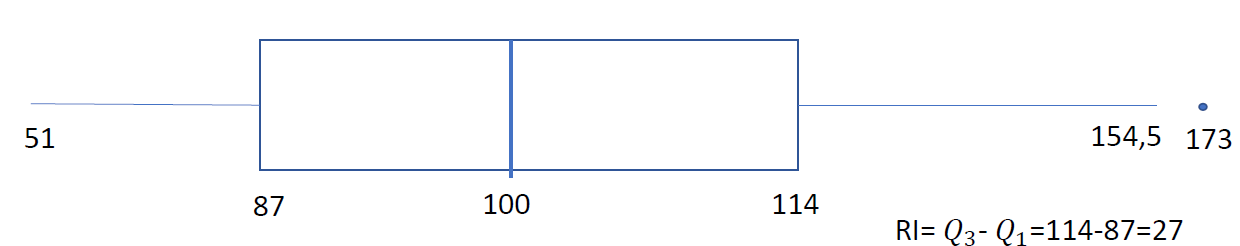
\includegraphics[width=0.9\textwidth]{boxplot.png}
	\end{figure}
	\[
	A_B = \frac{(Q_3 - Me) - (Me - Q_1)}{Q_3-Q_1} = \frac{14-13}{27} = \boxed{0.04} 
	\]
	No hay valores atípicos por la izquierda, pero vemos que el valor máximo es atípico por la derecha (173), pero no es un valor extremo ya que no supera $Q_3 + 3RI = 195$ \\
	Hay una ligera asimetría a la derecha poco significante \\  
	e) Calculamos el coeficiente de variación de Pearson para ver representatividad de la media
	\[
	CV_x = \frac{S_x}{\bar{x}} = \frac{22.06}{93.39} = 0.24
	\] 
	\[
	CV_y = \frac{S_y}{\bar{y}} = \frac{5.16}{55.66} = 0.09
	\]
	La media del numero de cetano es más representativa ya que la dispersión de la muestra es menor
	\section{Solución Problema 2}
	\begin{itemize}
		\item $\bar{x} = 6$
		\item $\bar{y} = 4$
		\item $b_{xy} = \frac{s_{xy}}{s_y^2} = 1.15$
		\item $b_{yx} = \frac{s_{yx}}{s_x^2} = 0.81$
		\item $CV_y = \frac{s_y}{\bar{y}} = 0.5 \rightarrow s_y = 0.5 \cdot 4 = 2 \rightarrow s_{xy} = 1.15 \cdot 2^2 = 4.6 \rightarrow s_x^2 = \frac{4.6}{0.81} = 5.68 \rightarrow s_x = 2.38$
	\end{itemize}
	a) Nos piden predecir las exportaciones de la empresa (Y) teniendo 25M de euros en ventas totales. Usamos una recta $Y | X$ \\
	\[
	y - \bar{y} = \frac{s_{xy}}{s_x^{2}} (x - \bar{x}) \rightarrow y - 4 = 0.81(x - 6) \rightarrow y = 0.81x - 0.86
	\]
	\[
	y = 0.81(25) - 0.86 = 19.39
	\]
	Las exportaciones serán 19.39M de euros por 25M de euros en ventas totales \\
	b)
	\[
	r = \frac{s_{xy}}{s_x \cdot s_y} = \frac{4.6}{2.38 \cdot 2} = \boxed{0.97}
	\]
	\[
	R^2 = r^2 = (0.97)^{2} = \boxed{94.09\%}
	\]
	Interdependencia directa muy fuerte: las exportaciones aumentan con las ventas totales \\
	Los valores teóricos están muy cerca de los observados \\
	Las predicciones tienen una fiabilidad del 94.09\% y el ajuste es muy bueno \\
	Las dos rectas de regresión son casi coincidentes \\
	c) Calculamos el coeficiente de variación de Pearson para ver representatividad de la media
	\[
	CV_x = \frac{S_x}{\bar{x}} = \frac{2.38}{6} = 0.4
	\] 
	\[
	CV_y = \frac{S_y}{\bar{y}} = \frac{2}{4} = 0.5
	\]
	La media de las ventas totales es más representativa ya que la dispersión de la muestra es menor \\
	d) Varianza residual: $s_y^2(1-r^2) = 4(1-0.9409) = 0.24$. Varianza explicada: $s_y^2 \cdot r^2 = 4 \cdot 0.9409 = 3.76$ \\
	Casi toda la variabilidad de las exportaciones queda explicada por las ventas totales. Solo 0.24 unidades de variabilidad no quedan explicadas.
	\section{Solución Problema 3}
	\begin{itemize}
		\item $\bar{x} = \frac{\sum_{i=1}^n x_i}{n} = \frac{7.1}{5} = 1.42$
		\item $\bar{y} = \frac{\sum_{i=1}^n y_i}{n} = \frac{131}{5} = 26.2$ 
		\item $s_x^{2} = \frac{\sum_{i=1}^n x_i^{2}}{n} - \bar{x}^{2} = \frac{15.565}{5} - 1.42^{2} = 1.1$ $s_x = 1.05$
		\item $s_y^{2} = \frac{\sum_{i=1}^n y_i^{2}}{n} - \bar{y}^{2} = \frac{5313}{5} - 26.2^{2} = 376.16$ $s_y = 19.4$
		\item $s_{xy} = \frac{\sum_{i=1}^n x_i y_i}{n} - \bar{x} \bar{y} = \frac{285.6}{5} - (1.42 \cdot 26.2) = 19.92$
	\end{itemize}
	a) Para saber si las variables están linealmente relacionadas, calculamos r
	\[
	r = \frac{s_{xy}}{s_x \cdot s_y} = \frac{19.92}{1.05 \cdot 19.4} = \boxed{0.98}
	\]
	\[
	R^2 = r^2 = (0.98)^{2} = \boxed{96.08\%}
	\]
	Interdependencia directa muy fuerte: la velocidad de reacción aumenta con la concentración de glucosa \\
	Los valores teóricos están muy cerca de los observados \\
	Las predicciones tienen una fiabilidad del 96.08\% y el ajuste es muy bueno \\
	Las dos rectas de regresión son casi coincidentes \\
	b) Nos piden predecir la concentración de glucosa a partir de una velocidad de 45 micromoles/minuto. Por lo tanto, usamos una recta de $X | Y$
	\[
	x - \bar{x} = \frac{s_{xy}}{s_y^{2}} (y - \bar{y}) \rightarrow x - 1.42 = 0.05(y - 26.2) \rightarrow x = 0.05y + 0.11
	\]
	\[
	x = 0.05(45) + 0.11 = 2.36
	\]
	La concentración de glucosa sera 2.36 milimoles/litro con una velocidad de 45 micromoles/minuto \\
	c) $b_yx = \frac{s_{xy}}{s_x^2} = \frac{19.92}{1.1} = 18.11$
	Por cada milimol/litro de glucogenosa, la velocidad de reacción aumenta 18.11 micromoles/minuto
	d)
	\[
	V_r = s_y^2 (1-r^2) = 376.16 \cdot (1-0.9608) = \boxed{14.9} 
	\]
	No quedan explicadas 14.9 unidades de varianza de la velocidad de reacción por la concentración de glucosa. Representan un 3.92\% de la variabilidad total \\
	f) $Q_1 = 10$, $Me = 18$, $Q_3 = 35$
	\begin{figure}[H]
		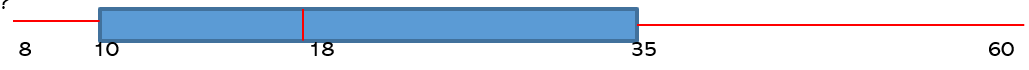
\includegraphics[width=0.9\textwidth]{boxplot2.png}
	\end{figure}
	Vemos que presenta asimetría hacia la derecha ya que $Q_3 - Me > Me - Q_1$. Por lo que la media es mayor que la mediana. Además, se evidencia que hay mayor dispersión en los valores más altos (35 - 60)
	\section{Solución Problema 4}
	\begin{itemize}
		\item $\bar{x} = \frac{\sum_{i=1}^n x_i}{n} = 28$
		\item $\bar{y} = \frac{\sum_{i=1}^n y_i}{n} = 0.414$ 
		\item $s_x^{2} = \frac{\sum_{i=1}^n x_i^{2}}{n} - \bar{x}^{2} = \frac{3958}{5} - 28^{2} = 7.6$ $s_x = 2.76$
		\item $s_y^{2} = \frac{\sum_{i=1}^n y_i^{2}}{n} - \bar{y}^{2} = \frac{0.86}{5} - 0.414^{2} = 0.0006$ $s_y = 0.02$
		\item $s_{xy} = \frac{\sum_{i=1}^n x_i y_i}{n} - \bar{x} \bar{y} = \frac{57.68}{5} - (28 \cdot 0.414) = -0.056$
	\end{itemize}
	a) Para saber si las variables están linealmente relacionadas, calculamos r
	\[
	r = \frac{s_{xy}}{s_x \cdot s_y} = -\frac{0.056}{2.76 \cdot 0.024} = \boxed{-0.82}
	\]
	\[
	R^2 = r^2 = (-0.82)^{2} = \boxed{67.24\%}
	\]
	Interdependencia inversa fuerte: la producción del trigo disminuye con el aumento del precio de harina \\
	Los valores teóricos están cerca de los observados \\
	Las predicciones tienen una fiabilidad del 67.24\% y el ajuste es bueno \\
	Las dos rectas de regresión son forman un ángulo pequeño \\
	b)  Nos piden predecir la produccion de trigo a partir de un precio de harina de 0.47 euros. Por lo tanto, usamos una recta de $X | Y$
	\[
	x - \bar{x} = \frac{s_{xy}}{s_y^{2}} (y - \bar{y}) \rightarrow x - 28 = -2.28(y - 0.414) \rightarrow x = -2.28y + 28.94
	\]
	\[
	x = -2.28(0.47) + 28.94 = 27.86
	\]
	La producción de trigo serán 27.86 Tm con un precio de harina de 0.47 euros \\
	c) $b_yx = \frac{s_{xy}}{s_x^2} = -\frac{0.056}{7.6} = -0.0074$ \\
	Por cada Tm de trigo, el precio de la harina disminuye 0.0074 euros \\
	d) \\
	\begin{table}[h!]
		\centering
		\begin{tabular}{|c|c|c|c|c|}
			\hline
			\( x_i \) & 25 & 28 & 30 & 32 \\ \hline
			\( n_i \) & 2 & 1 & 1 & 1 \\ \hline
		\end{tabular}
	\end{table}
	
	El 50\% central estará entre 25 y 28 Tm 
	\section{Solución Problema 5}
	\begin{itemize}
		\item $\bar{x} = \frac{\sum_{i=1}^n x_i}{n} = \frac{50.1}{5} = 10.02$
		\item $\bar{y} = \frac{\sum_{i=1}^n y_i}{n} = \frac{125}{5} = 25$ 
		\item $s_x^{2} = \frac{\sum_{i=1}^n x_i^{2}}{n} - \bar{x}^{2} = \frac{614.21}{5} - 10.02^{2} = 22.44$ $s_x = 4.74$
		\item $s_y^{2} = \frac{\sum_{i=1}^n y_i^{2}}{n} - \bar{y}^{2} = \frac{3753}{5} - 25^{2} = 125.6$ $s_y = 11.21$
		\item $s_{xy} = \frac{\sum_{i=1}^n x_i y_i}{n} - \bar{x} \bar{y} = \frac{1514.6}{5} - (10.02 \cdot 25) = 52.42$
	\end{itemize}
	a) Para saber si las variables están linealmente relacionadas, calculamos r
	\[
	r = \frac{s_{xy}}{s_x \cdot s_y} = \frac{52.42}{11.21 \cdot 4.74} = \boxed{0.98}
	\]
	\[
	R^2 = r^2 = (0.98)^{2} = \boxed{96.04\%}
	\]
	Interdependencia directa muy fuerte: el tiempo que tarda aumenta con la distancia \\
	Los valores teóricos están muy cerca de los observados \\
	Las predicciones tienen una fiabilidad del 96.04\% y el ajuste es muy bueno \\
	Las dos rectas de regresión son casi coincidentes \\
	b) Nos piden predecir el tiempo que tarda a partir de que vive a 14km de distancia. Por lo tanto, usamos una recta de $Y | X$
	\[
	y - \bar{y} = \frac{s_{xy}}{s_x^{2}} (x - \bar{x}) \rightarrow y - 25 = 2.34(x - 10.02) \rightarrow y = 2.34x + 1.55
	\]
	\[
	y = 2.34(14) + 1.55 = 34.31
	\]
	El tiempo que tarda será de 34.31 minutos viviendo a 14km de distancia\\
	c)  Calculamos el coeficiente de variación de Pearson para ver representatividad de la media y dispersión
	\[
	CV_x = \frac{S_x}{\bar{x}} = \frac{4.74}{10.02} = 0.47
	\] 
	\[
	CV_y = \frac{S_y}{\bar{y}} = \frac{11.21}{25} = 0.45
	\]
	La media del tiempo es más representativa ya que la dispersión de la muestra es menor \\
	d) 
	\[
	V_r = s_y^2 (1-r^2) = 125.6 \cdot (1-0.9604) = \boxed{4.97} 
	\]
	No quedan explicadas 4.97 unidades de varianza del tiempo de llegada por la distancia. Representan un 3.94\% de la variabilidad total \\
	\section{Solución Problema 6}
	\begin{itemize}
		\item $\bar{x} = \frac{\sum_{i=1}^n x_i}{n} = \frac{288}{5} = 57.6$
		\item $\bar{y} = \frac{\sum_{i=1}^n y_i}{n} = \frac{11}{5} = 2.2$ 
		\item $s_x^{2} = \frac{\sum_{i=1}^n x_i^{2}}{n} - \bar{x}^{2} = \frac{16612}{5} - 57.6^{2} = 4.64$ $s_x = 2.15$
		\item $s_y^{2} = \frac{\sum_{i=1}^n y_i^{2}}{n} - \bar{y}^{2} = \frac{31}{5} - 2.2^{2} = 1.36$ $s_y = 1.17$
		\item $s_{xy} = \frac{\sum_{i=1}^n x_i y_i}{n} - \bar{x} \bar{y} = \frac{623}{5} - (57.6 \cdot 2.2) = -2.12$
		\item $r = \frac{s_{xy}}{s_x \cdot s_y} = -\frac{2.12}{2.15 \cdot 1.17} = -0.84$
		\item $R^2 = r^2 = (-0.84)^{2} = 70.56\%$
	\end{itemize}
	a) Nos piden predecir el diámetro de un neumático con 0 pinchazos. Por lo tanto, usamos una recta de $X | Y$
	\[
	x - \bar{x} = \frac{s_{xy}}{s_y^{2}} (y - \bar{y}) \rightarrow x - 57.6 = -1.81(y - 2.2) \rightarrow x = -1.81y + 61.58
	\]
	\[
	x = -1.81(0) + 61.58 = 61.58
	\]
	El diámetro será de 61.58 cm con 0 pinchazos. Hay un grado de fiabilidad del 70.56\% \\
	b) Calculamos el coeficiente de variación de Pearson para ver representatividad de la media y dispersión
	\[
	CV_x = \frac{S_x}{\bar{x}} = \frac{2.15}{57.6} = 0.04
	\] 
	\[
	CV_y = \frac{S_y}{\bar{y}} = \frac{1.17}{2.2} = 0.53
	\]
	La media del diámetro es más representativa ya que la dispersión de la muestra es menor \\
	c) Dado que $r = -0.84$ y $R^2 = 70.56\%$ podemos interpretar que: \\
	Interdependencia inversa fuerte: el diámetro disminuye cuando el numero de pinchazos aumenta \\
	Los valores teóricos están cerca de los observados \\
	Las predicciones tienen una fiabilidad del 70.56\% y el ajuste es bueno \\
	Las dos rectas de regresión forman un ángulo pequeño \\
	d)
	\[
	V_expl = s_y^2 (r^2) = 1.36 \cdot 0.7056 = \boxed{0.96} 
	\]
	Quedan explicadas 0.96 unidades de varianza del diámetro del neumático por el numero de pinchazos. Representan un 70.56\% de la variabilidad total \\
	\section{Solución Problema 7}
	\begin{itemize}
		\item $\bar{x} = \frac{\sum_{i=1}^n x_i}{n} = \frac{509}{5} = 101.8$
		\item $\bar{y} = \frac{\sum_{i=1}^n y_i}{n} = \frac{69}{5} = 13.8$ 
		\item $s_x^{2} = \frac{\sum_{i=1}^n x_i^{2}}{n} - \bar{x}^{2} = \frac{52855}{5} - 101.8^{2} = 207.76$ $s_x = 14.41$
		\item $s_y^{2} = \frac{\sum_{i=1}^n y_i^{2}}{n} - \bar{y}^{2} = \frac{1095}{5} - 13.8^{2} = 28.56$ $s_y = 5.34$
		\item $s_{xy} = \frac{\sum_{i=1}^n x_i y_i}{n} - \bar{x} \bar{y} = \frac{7017}{5} - (101.8 \cdot 13.8) = -1.44$
		\item $r = \frac{s_{xy}}{s_x \cdot s_y} = -\frac{1.44}{14.41 \cdot 5.34} = -0.02$
		\item $R^2 = r^2 = (-0.02)^{2} = 0.04\%$
	\end{itemize}
	a) Nos piden predecir el número de semanas en cartel a partir de que la película dura 2 horas. Por lo tanto, usamos una recta de $Y | X$
	\[
	y - \bar{y} = \frac{s_{xy}}{s_x^{2}} (x - \bar{x}) \rightarrow y - 13.8 = -0.007(x - 101.8) \rightarrow y = -0.007x + 14.51
	\]
	\[
	y = -0.007(2) + 14.51 = 14.49
	\]
	El número de semanas en cartel será de 14.49 si la película dura 2 horas. Tiene una fiabilidad del 0.04\% \\
	b) 	\[
	V_r = s_y^2 (1-r^2) = 28.56 \cdot (1-0.0004) = \boxed{28.55} 
	\]
	No quedan explicadas 28.55 unidades de varianza de las semanas en cartel por la duración de la película. Representan un 99.96\% de la variabilidad total \\
	c) Dado que $r = -0.02$ y $R^2 = 0.04\%$ podemos interpretar que: \\
	Interdependencia inversa muy débil (casi nula): el número de semanas disminuye cuando el numero de minutos de la película aumenta \\
	Los valores teóricos están muy lejos de los observados \\
	Las predicciones tienen una fiabilidad del 0.04\% y el ajuste es pésimo \\
	Las dos rectas de regresión forman un ángulo casi perpendicular \\
\end{document}